\section{Framework}\label{ss:framework}

In this section, we present the components of our framework for assessing static and dynamic personalization, including details for fitting a hierarchical Bayesian PK model to concentration data from a cohort of patients, assessing the behaviour of Markov chains via diagnostics, and using the Bayesian model to generate simulated data for evaluation. We then outline several modes of static and dynamic personalization ranging from no personalization (every patient gets the same dose) to a complex dynamic mode of personalization (estimation of the optimal Dynamic Treatment Regime for dosing).  Finally, we outline steps for assessing the benefits of each mode of personalization.

\subsection{Bayesian Modelling}

The first step in our framework is to fit a Bayesian model that relates patient covariates and dose to drug concentration as a function of time. For example, previous work \cite{pananos2020comparisons} describes a hierarchical Bayesian model of apixaban pharmacokinetics, in which the clearance $Cl$ (L/hour), time to maximum concentration $t_{max}$ (hours), absorption time delay $\delta$ (hours), and ratio between the elimination and absorption rate constants ($\alpha = k_e/k_a$, a unitless parameter) are hierarchically modelled. In our case study, we extend that model by regressing the latent pharmacokinetic parameters on baseline clinical variables (age, sex, weight, and creatinine) to permit personalization. The model could equally well be extended with pharmacokinetic or biomarker information if the relevant theory and data were available for a particular use case. We detail our hierarchical Bayesian pharmacokinetic model and provide sampler diagnostics in \cref{ap:appendix}.


\subsection{Modes of Personalization \& Assessment of Personalization}

The second step in our framework is to identify modes of personalization that we wish to evaluate. We classify these modes of personalization into two types: static and dynamic personalization.

Static modes of personalization seek to inform the dose at one point in time (usually treatment initiation) with the goal of eliminating the need for ``trial-and-error'' adjustments.  We consider two modes of static personalization in our case study:

\begin{enumerate}
	\item \textbf{One size fits all}.  This mode of personalization is not very personal at all.  All patients receive the same dose size at the onset of treatment ($\approx8.5 mg$ taken twice daily). This dose was selected so that the average value across patients was maximized.  
	\item \textbf{Dose based on clinical variables}.  In this mode of personalization, the patient's covariates, for example age, sex, weight, creatinine (a measure of kidney function )measurements, and possibly genetic or biomarker information, are provided to the pharmacokinetic model.  A dose size is then selected using the model to maximize the value function conditional on these measurements.
\end{enumerate}

\noindent Dynamic modes of personalization seek to personalize the initial doses but also the titration process.  We consider four modes of dynamic personalization for our case study:

\begin{enumerate}
	\item \textbf{One size fits all initial dose \textit{and} one dose adjustment}.  This mode of personalization provides patients the same dose to start, but requires a concentration measurement to be made sometime in the future, which is then used to adjust the dose.  For example, in our case study, patients take their initial dose once every 12 hours with perfect adherence for five days, and, a sample is taken randomly in the second 12 hour period of the fourth day.  Our pharmacokinetic model conditions on this measurement, and the dose is adjusted in order to maximize the reward for another five days by updating our Bayesian model with the measurement.
	
	\item \textbf{Initial dose based on clinical variables \textit{and} one dose adjustment}.  Here, the initial dose provided to the patient is determined by the patient's clinical measurements. For example, in our case study, in the second half of the fifth day, a concentration measurement is made at a random time. The model is conditioned on this concentration and the dose is adjusted to optimize the reward.
	
	\item \textbf{Initial dose based on clinical variables \textit{and} optimally-timed observation}.  Similar to the previous mode of personalization, but the time at which the measurement is made is under our control and tuned to maximize reward. The time at which the sample is taken can yield more or less information about particular parameters in the model, but increases the burden by necessitating an additional constraint on when the observation should be obtained. For example, measuring much later after the dose is taken yields more information about the elimination rate constant $k_e$ than it does about the absorption rate constant $k_a$ because later in time, the majority of the dose has been absorbed and is now being eliminated by the body. In this mode of personalization, the initial dose and the timing of the adjustment are optimized independently. 
	
	\item \textbf{Optimal sequential dosing}. The approach of this mode is the same as the previous mode, except that the initial dose and the timing of the adjustment are \textit{jointly optimized} using Q-learning to maximize the expected reward.
\end{enumerate}
We stress that these are just examples of some modes of personalization, and that we do not mean that these modes should always be candidate modes for personalization, nor that they are the only modes of interest.  These modes may not be appropriate for all drugs across all indications, and were selected in order to illustrate natural extensions and combinations of static personalization with additional information collection. A strength of our approach is that many possible modes of personalization may be considered depending on what is appropriate for the use-case at hand.

Each simulated patient has their dose(s) selected under each mode of personalization.  Since the patients are simulated, we can compute what the return under the proposed dose(s) obtained from each mode of personalization and compare the return achieved to the largest return theoretically possible (i.e.\ the return achieved were we to know the pharmacokinetic parameters exactly when providing the initial dose, which is not possible in practice). The difference between this optimal return and the actual return is called the \textit{regret}. Comparing the regrets achieved by different modes allows us to assess their relative performance, and helps us decide which are most appropriate for a given personalized medicine problem.

\begin{figure}
	\centering
	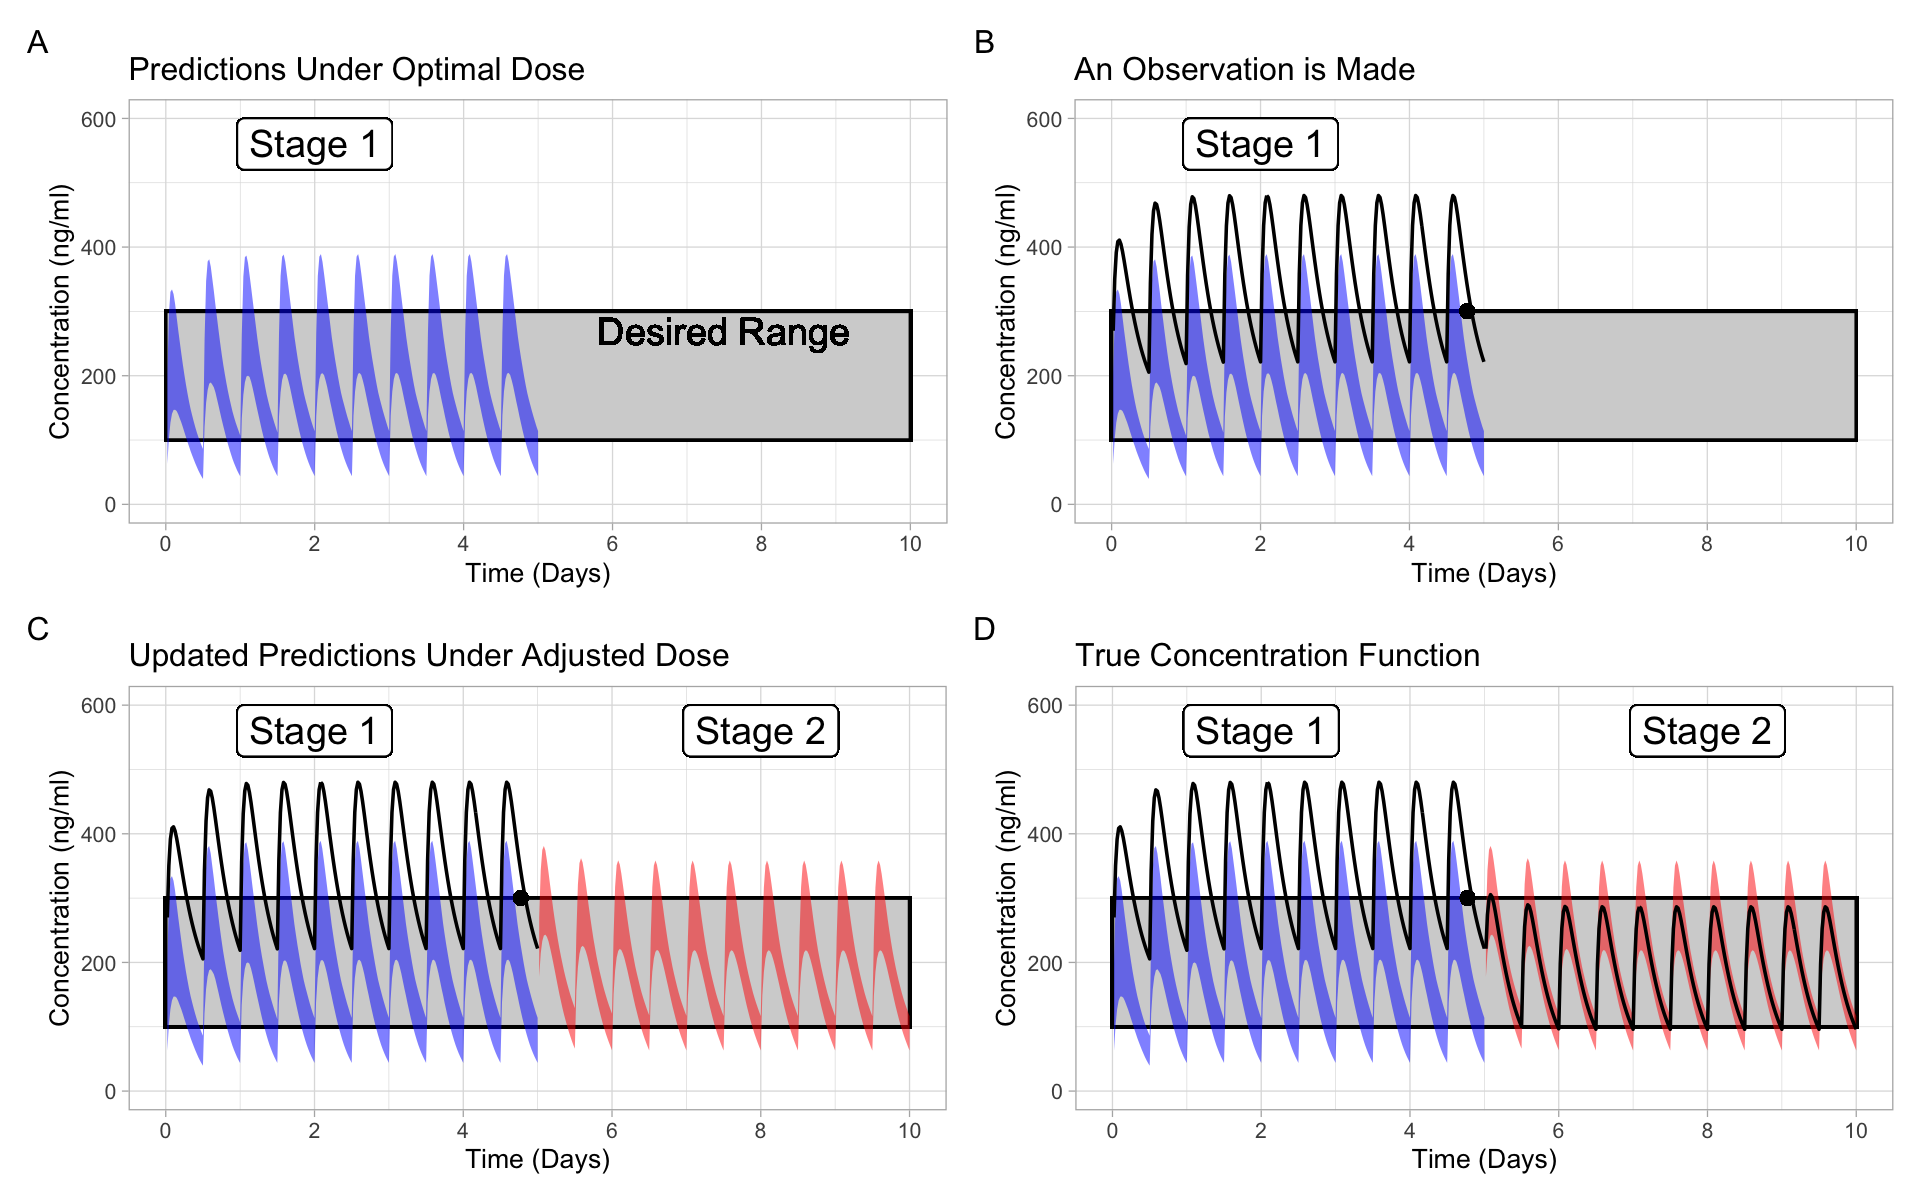
\includegraphics[width=1\linewidth]{figures/viz_of_process.png}
	\caption{
	Visual representation of the steps in our framework.	\textbf{A}  Using only clinical information, the model is used to select a dose that is expected to keep the patient in the desired range for as long as possible. The blue ribbon indicates 90\% credible interval for the latent concentration.  \textbf{B} Some time later, the patient's blood serum concentration is measured (black dot). \textbf{C}  The observation is incorporated into the model and a new dose is selected to keep the patient in range for as long as possible. The red ribbon indicates 90\% credible interval for the latent concentration after adjusting the dose. \textbf{D} The black line indicates the true latent concentration under each dose.  Note the observation (black dot) is not on the black line (true concentration) because there is measurement error, which the model accounts for.
	%Black exes indicate a discretization use to compute the reward function in each stage.
    % ^^^ I don't see these any more - maybe they are no longer used?
}
	\label{fig:processfiguresingle}
\end{figure}

